\documentclass[12pt]{article}
\usepackage{tabularx}
\usepackage{graphicx}
\usepackage{adjustbox}

\usepackage[headheight=26pt, textheight=7in, footskip=20pt]{geometry}% http://ctan.org/pkg/geometry

\usepackage{lipsum}% http://ctan.org/pkg/lipsum
\usepackage{fancyhdr}% http://ctan.org/pkg/fanychdr
\usepackage{lastpage}
\newcommand{\myboxp}[1]{
\noindent\fbox{
    \parbox[t][]{14.5cm}{
        #1
    }
}~\\~\\~\\
}
\newcolumntype{P}[1]{>{\centering\arraybackslash}p{#1}}
\def\arraystretch{1.5}
\fancypagestyle{myheader}{%
  \fancyhf{}% clear header/footer
  \fancyhead[L]{
    \begin{tabular}{|P{7.1cm}|P{7.1cm}|}
            \hline
            ~ & ~ \\
            \includegraphics[width=5cm]{/home/unaj/unaj-header.png} & Pr\'{a}ctica Profesional Supervisada \\
            Instituto de Ingenier\'{i}a y Agronom\'{i}a Ingenier\'{i}a en Inform\'{a}tica  & \textbf{(PPS)} \\
            ~ & \multicolumn{1}{r|}{P\'{a}gina~\thepage~de~\pageref{LastPage}} \\
            \hline
        \end{tabular}
  }
  \renewcommand{\headrulewidth}{0pt}% No header rule
  \renewcommand{\footrulewidth}{0pt}% No footer rule
}
\setlength{\headheight}{126pt}
\pagestyle{myheader}



\usepackage{indentfirst}
\usepackage{framed}
\usepackage{mathptmx}
\usepackage{csquotes}
\usepackage{float}
\linespread{1.241}
\usepackage[utf8]{inputenc}
\usepackage[backend=biber, style=apa, autocite=inline, hyperref=false]{biblatex}
\DeclareLanguageMapping{spanish}{spanish-apa}
\usepackage{graphicx}
\addbibresource{bibliografia.bib}
\usepackage{caption}
\usepackage{color}
\captionsetup{
    justification=raggedright,singlelinecheck=false, labelfont=bf
}
\usepackage{hyperref}
\hypersetup{
    urlcolor=blue,
    colorlinks=true,
    citecolor=blue,
    linkcolor=black
}
\usepackage[spanish]{babel}
\usepackage[T1]{fontenc}
\usepackage{listings}
\usepackage{xcolor}
\definecolor{codegreen}{rgb}{0,0.6,0}
\definecolor{codegray}{rgb}{0.5,0.5,0.5}
\definecolor{codepurple}{rgb}{0.58,0,0.82}
\definecolor{backcolour}{rgb}{0.95,0.95,0.92}

\lstdefinestyle{mystyle}{
    backgroundcolor=\color{backcolour},
    commentstyle=\color{codegreen},
    keywordstyle=\color{magenta},
    numberstyle=\tiny\color{codegray},
    stringstyle=\color{codepurple},
    basicstyle=\ttfamily\footnotesize,
    breakatwhitespace=false,
    breaklines=true,
    captionpos=b,
    keepspaces=true,
    numbers=left,
    numbersep=5pt,
    showspaces=false,
    showstringspaces=false,
    showtabs=false,
    tabsize=2,
    morekeywords={
        fos_user:,
        resource:,
        db_driver:,
        firewall_name:,
        user_class:,
        group:,
        group_class:,
        group_manager:,
        service:,
        user_manager:,
        from_email:,
        address:,
        sender_name:,
        sonata_user:,
        manager_type:,
        sonata_user_admin_security:,
        sonata_user_admin_resetting:,
        admin:,
        pattern:,
        context:,
        form_login:,
        provider:,
        login_path:,
        use_forward:,
        check_path:,
        failure_path:,
        default_target_path:,
        logout:,
        path:,
        target:,
        anonymous:,
        main:,
        role_hierarchy:,
        ROLE_ADMIN:,
        ROLE_SUPER_ADMIN:,
        SONATA:,
        providers:,
        fos_userbundle:,
        id:,
        encoders:,
        access_control:,
        class:,
        user:
    }
}


\renewcommand*{\lstlistingname}{Ejemplo de código}

\renewcommand{\arraystretch}{1.5}

\lstset{
    style=mystyle,
    alsoletter={:}
}


\author{Franco Ganga}
\title{Proyecto\ RUDA:\ Registro\ unificado\ de\ actividades}

\def\signed #1{{\leavevmode\unskip\nobreak\hfil\penalty50\hskip2em
  \hbox{}\nobreak\hfil(#1)%
  \parfillskip=0pt \finalhyphendemerits=0 \endgraf}}

\newsavebox\mybox
\newenvironment{aquote}[1]
  {\savebox\mybox{#1}\begin{quote}}
  {\signed{\usebox\mybox}\end{quote}}


\setlength{\parindent}{1cm}


\newcommand{\myparagraph}[1]{\paragraph{#1}\mbox{}\\}

\newcommand{\sonatainstallation}{https://sonata-project.org/bundles/user/master/doc/reference/installation.html}



\begin{document}
\centerline{\large{PRÁCTICA PROFESIONAL SUPERVISADA (PPS)}}
\centerline{\large{Registro Unificado de Actividades}}
\centerline{\large{Informe Final}}
\begin{framed}
        \noindent\textbf{DATOS DEL ESTUDIANTE}\newline
        Apellido y Nombres: Ganga Franco Manuel\newline
        DNI: 37837656\newline
        Nº de Legajo: 3917\newline
        Correo electr\'{o}nico: fganga@ymail.com\newline
        Cantidad de materias aprobadas al comienzo de la PPS: 45\newline
        PPS enmarcada en art\'{i}culo: 4 \newline
        Periodo en que se realiz\'{o} la PPS: Año 2019
\end{framed}

\begin{framed}
        \noindent\textbf{DOCENTE SUPERVISOR}  \newline
        Apellido y Nombres: Morales Martín \newline
        Correo electr\'{o}nico: martin.morales@unaj.edu.ar
\end{framed}

\vfill
\noindent\begin{tabular}{|P{3.3cm}|P{3.3cm}|P{3.3cm}|P{3.3cm}|}
\hline
Firma Estudiante: & Firma Docente Supervisor: & Firma docente tutor TAPTA: & Firma tutor Organizacional: \\
~ & ~ & ~ & ~ \\
~ & ~ & ~ & ~ \\
\hline
\end{tabular}
\newpage

\begin{framed}
        \noindent\textbf{DOCENTE  TUTOR DEL TALLER DE APOYO A LA PRODUCCI\'{O}N DE TEXTOS ACAD\'{E}MICOS DE LA UNAJ}\newline
        Apellido y Nombres: Lavigna Lia \newline
        Correo electr\'{o}nico: lialavigna@gmail.com
\end{framed}

\begin{framed}
\noindent\textbf{DATOS DE LA ORGANIZACI\'{O}N DONDE SE REALIZA LA PPS}\newline
Nombre o Raz\'{o}n Social: Universidad Nacional Arturo Jauretche\newline
Direcci\'{o}n: Av. Calchaquí 6200\newline
Tel\'{e}fono: 4275-6100 \newline
Sector: Informática
\end{framed}

\begin{framed}
\noindent\textbf{TUTOR DE LA ORGANIZACIONAL}\newline
Apellido y Nombres: Gustavo Pilla \newline
Correo electr\'{o}nico: gpilla@unaj.edu.ar
\end{framed}

\begin{framed}
    \noindent\textbf{FIRMA DEL COORDINADOR DE LA CARRERA}
\end{framed}
\vfill
\noindent\begin{tabular}{|P{3.3cm}|P{3.3cm}|P{3.3cm}|P{3.3cm}|}
\hline
Firma Estudiante: & Firma Docente Supervisor: & Firma docente tutor TAPTA: & Firma tutor Organizacional: \\
~ & ~ & ~ & ~ \\
~ & ~ & ~ & ~ \\
\hline
\end{tabular}
\newpage

\tableofcontents
\newpage

\section{Desarrollo}%
\label{sec:desarrollo}


\subsection{Introducción Symfony}%
\label{ssub:introduccion_symfony}
Symfony es un \textit{framework} PHP de código abierto para desarrollar aplicaciones web. Originalmente fue concebido por la
agencia interactiva SensioLabs para el desarrollo de sitios web para sus propios clientes. Symfony se publicó en 2005 bajo
la licencia MIT Open Source y hoy se encuentra entre los principales \textit{frameworks} disponibles para el desarrollo de PHP. \parencite{symfony-def}


Un proyecto Symfony está conformado por varios componentes que proveen funciones básicas para una aplicación web. Entender
el funcionamiento de cada uno de ellos es necesario para una buena implementación\@. Para el desarrollo del presente proyecto se utilizaron los siguientes componentes de Symfony:


\begin{itemize}
    \item \textbf{Asset:} administra la generación de URL y el versionado de hojas de estilo css, archivos JavaScript e imágenes.
\item \textbf{Console:} permite crear comandos para usar en consola. Bastante útil para tareas recurrentes.
\item \textbf{Dotenv:} administra las variables de entorno de la aplicación.
\item \textbf{Expression Language:} permite utilizar expresiones dentro de archivos de configuración para obtener lógica más compleja.
\item \label{itm:flex} \textbf{Flex:} es un componente que facilita la integración de paquetes de terceros a través de lo que se denomina recetas Symfony. Estas recetas consisten en un conjunto de instrucciones automatizadas.
\item \textbf{Form:} permite crear, procesar y reutilizar formularios.
\item \textbf{Framework:} define la configuración principal del framework.
\item \textbf{Monologbundle:} integra la librería monolog con symfony para el registro de mensajes.
\item \textbf{ORM Pack:} es la librería encargada del mapeo objeto-relacional.
\item \textbf{Process:} librería utilizada para la ejecución de subprocesos. Resuelve problemas relacionados con la diferencia entre sistemas operativos y además provee una ejecución segura.
\item \textbf{Security:} componente de seguridad de Symfony. Se encarga de definir el control de acceso, sistemas de autenticación y además de establecer los proveedores de usuarios.
\item \textbf{Serializer:} paquete de Symfony que se encarga de transformar un objeto en un formato adecuado para la transmisión de datos. Ej: JSON.
\item \textbf{Swiftmailer:} permite el envío de emails a través de un servidor propio o de terceros.
\item \textbf{Translation:} permite definir textos en la aplicación para traducción al idioma local del usuario. Este proceso es comúnmente llamado internacionalización.
\item \textbf{Twig:} Motor de templates preferido por Symfony, permite renderizar contenido html de manera fácil, organizada y segura.
\item \textbf{Validator:} componente encargado de la validación de datos. Weblink: incrementa la performance de la aplicación al utilizar HTTP2 y funciones de precarga en navegadores modernos.
\item \textbf{Yaml:} se encarga de convertir archivos YAML en arrays PHP. Gran parte de la configuración de Symfony se encuentra definida en este formato.

\end{itemize}
\newpage


\subsection{Modelado}%
\label{sub:modelado}
En primer lugar, se definieron relaciones básicas de acuerdo a los requerimientos del sistema para poder crear las clases admin y definir las entidades como
recursos \textit{API-Platform}.

\subsubsection{Introducción a Doctrine}%
\label{ssub:introducción_doctrine}
Con Doctrine, cada objeto PHP que se requiera persistir a la base de datos, necesita estar definido en un archivo PHP que
contiene información referente a tipos de dato y relaciones entre entidades. A este archivo se lo denomina entidad.

\begin{figure}[H]
    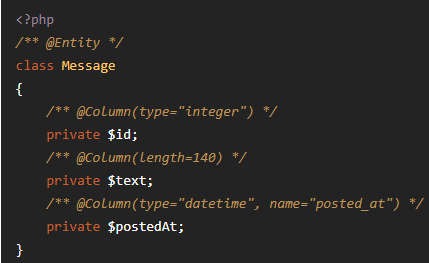
\includegraphics[width=1\linewidth]{image/entidad-doctrine.png}
    \caption[Ejemplo básico de una entidad]{Ejemplo básico de una entidad.\newline \textbf{Fuente:} Recuperado de \url{www.doctrine-project.org/
    projects/doctrine-orm/en/2.6/reference/basic-mapping.html}}%
    \label{fig:image/entidad-doctrine}
\end{figure}
Una relación en \textbf{Doctrine} está formado por dos entidades. Una de ellas actúa como el lado propietario de la relación y la otra como el inverso\@.
El lado propietario de la relación es aquel en el que \textbf{Doctrine} verifica si hubo cambios.
Existen dos tipos de mapeo de relaciones, bi-direccionales y uni-direccionales\@.
Una relación bi-direccional permite que ambos lados de la relación puedan accederse entre sí\@. En cambio, una relación uni-direccional sólo puede accederse
a través del lado propietario\@.
Al trabajar con relaciones, se debe tener en cuenta la manera en que Doctrine comprueba por cambios en los datos, ya que cambios persistidos en el lado
inverso de la relación serán ignorados por el ORM al momento de actualizar información a la base de datos.



\subsubsection{Actividad}%
\label{ssub:actividad}
Se modeló el siguiente esquema de acuerdo a la información recibida por parte del Área de Informática de la universidad\@.
Además, se pensó en utilizar herencia para la definición de las actividades, de esta manera cada cargo o actividad en particular
heredaría toda característica común de una entidad padre.

\begin{figure}[H]
    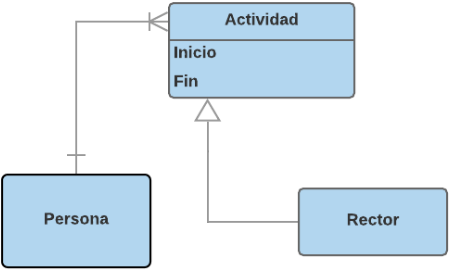
\includegraphics[scale=1]{image/actividad-modelo.png}
    \caption[Ejemplo de la definición de un cargo]{Ejemplo de la definición de un cargo.\newline \textbf{Fuente:} Elaboración propia}%
    \label{fig:image/actividad-modelo}
\end{figure}
El primer paso realizado para la definición de cada cargo o actividad fue la creación de la entidad \textit{Actividad}, la cual contendrá
datos de la persona relacionada y el periodo de desarrollo de la actividad o cargo\@.
Se agregó la función de Soft delete o borrado lógico, la que permite que, al borrar una actividad desde la aplicación web,
la misma es ocultada del usuario y no borrada de la base de datos\@. Esta función posibilita almacenar datos históricos del sistema\@.
Además, se agregó la función de Time stamps o etiquetas de tiempo, la cual hace posible el seguimiento de las fechas de creación
y actualización de cada actividad.


Se definió el mapeo de esta entidad en Doctrine mediante herencia de clase, una estrategia en la que cada clase en la jerarquía es mapeada a varias tablas:
la propia y las de todas las clases padre. La tabla de una clase hija es vinculada a la del padre a través de una clave foránea.

Doctrine implementa esta estrategia a través del uso de una columna denominada discriminator en la tabla más alta en la jerarquía\@. Esta es la mejor
manera de lograr consultas polimórficas con herencia de clase\@. \parencite{doctrine-inheritance}\\
\noindent
Esta columna identifica el tipo de entidad, por ejemplo: una
fila con un valor de ``director instituto'' significa que es una actividad del tipo DirectorInstituto\@.
Si no se provee el mapeo correspondiente, doctrine lo generará automáticamente utilizando el nombre de cada clase entidad en minúscula\@. \parencite{doctrine-inheritance}

\begin{figure}[H]
    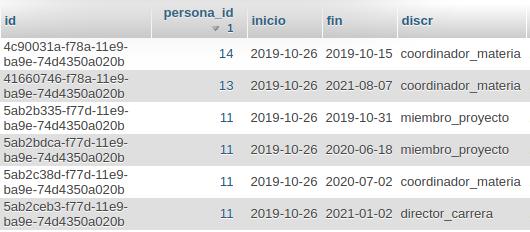
\includegraphics[width=1\linewidth]{image/discriminator-doctrine.png}
    \caption[Columna \textbf{discr} utilizada como discriminator]{Columna \textbf{discr} utilizada como discriminator.\newline \textbf{Fuente:} Elaboración propia, impresión de pantalla del código fuente.}
    \label{fig:image/discriminator-doctrine.png}
\end{figure}
\newpage
Se agregó la correspondiente metadata de la herencia en \textit{Actividad} y se optó por proporcionar el mapeo de la columna discriminator:

\begin{figure}[h]
    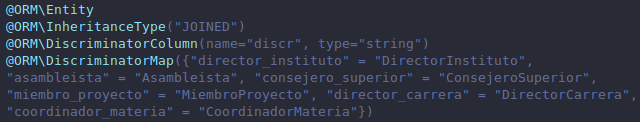
\includegraphics[width=1\linewidth]{image/discr.png}
    \caption[Mapeo de la columna \textbf{discriminator}]{Mapeo de la columna \textbf{discriminator}.\newline \textbf{Fuente:} Elaboración propia, impresión de pantalla del código fuente.}
    \label{fig:image/discr.png}
\end{figure}

\subsubsection{Miembro de Proyecto}%
\label{ssub:miembro_de_proyecto_modelo}
Esta entidad es la que almacenará datos acerca de la acción de formar parte de un proyecto. Cada dato de la columna \textbf{MiembroProyecto} representará la participación
de una persona a un proyecto\@.
Se mapeó la relación entre \textit{miembros} y \textit{proyectos} con una cardinalidad de 1-n y, dado que en este tipo de relaciones el lado n toma la clave foránea, el lado
propietario termina siendo \textit{miembros de proyecto}\@.
Con \textit{roles} sucede lo mismo, ya que cada instancia de miembro debe poseer un solo rol.

\begin{figure}[h]
    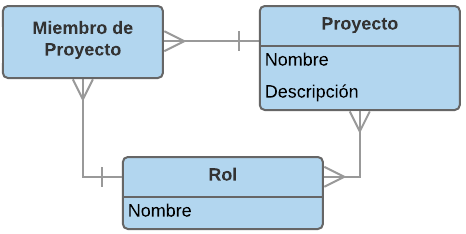
\includegraphics[width=1\linewidth]{image/mpr-new.png}
    \caption[Diagrama que representa la relación entre miembro, rol y proyecto]{Diagrama que representa la relación entre miembro, rol y proyecto.\newline \textbf{Fuente:} Elaboración propia utilizando una herramienta online de elaboración de diagramas.}
    \label{fig:image/mpr-new}
\end{figure}

\begin{figure}[h]
    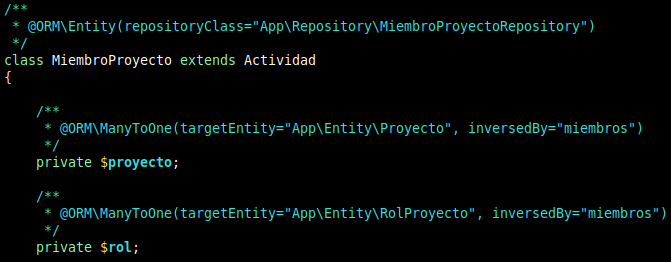
\includegraphics[width=1\linewidth]{image/miembros.png}
    \caption[Metadata de mapeo de relaciones de miembro de proyecto]{Metadata de mapeo de relaciones de miembro de proyecto.\newline \textbf{Fuente:} Elaboración propia.}
    \label{fig:image/miembros}
\end{figure}

\subsubsection{Proyecto}%
\label{ssub:modelo_proyecto}
En el sistema se necesita representar dos tipos de proyectos, de extensión y de investigación\@. Por ende, se decidió agregar \textbf{herencia} para la definición
de cada proyecto\@. Esto evita tener que crear una nueva entidad para representar los miembros del otro proyecto\@. De la misma forma que con Actividad se utilizó
herencia de clase.


En cuanto a sus relaciones, posee la relación con miembros desde el punto de vista de Proyecto. Con una cardinalidad de n-1 y siendo \textbf{Proyecto} el lado
inverso de la relación.

Por otro lado, también se definió su relación con \textbf{Roles de Proyecto} con una cardinalidad de n-n.

\subsubsection{Rol de Proyecto}%
\label{ssub:rol_de_proyecto_modelo}
Esta entidad representa un rol de proyecto, a cada instancia de miembro se le puede asignar un rol a ejercer en el Proyecto.

Se estableció la relación de roles del tipo n-n, es decir, con una cardinalidad de muchos a muchos; ya que un proyecto puede tener muchos roles y además
un rol puede tener muchos proyectos\@. Como la entidad de roles se actualizará a partir de los proyectos, se definió a Proyecto como dueño o propietario de
la relación. En el caso de una relación de este tipo el lado propietario es aquel que contiene el parámetro \textbf{inversedBy} en
su definición.~\parencite{doctrine-inheritance}



\subsection{Definición de ABMs - Clases Admin}%
\label{sub:definición_de_abms_clases_admin}

Para definir un ABM, es decir, una interfaz capaz de manejar el alta, baja y modificación de registros es necesario una entidad. Por este motivo, para obtener
una idea general del funcionamiento de Sonata-Admin, se decidió definir algunas entidades y generar una clase admin\@.
En sonata admin, una clase admin es aquella que, dada una entidad, permite añadir un servicio en la plataforma web sonata que se hace cargo de cada una de estas funciones.

Para crear un admin es necesario extender de la clase \textbf{AbstractAdmin} que provee sonata y, mediante métodos heredados de la misma, configurar la manera en
que se muestra la información\@.
Algunos de estos métodos son:

\begin{itemize}
    \item \textit{configureFormFields:} este método define los campos a mostrarse durante la acción de crear y editar.
    \item \textit{configureListFields:} define los campos a mostrar durante la acción de listar datos.
    \item \textit{configureShowFields:} establece la información a mostrar durante la acción de ver una entrada.
\end{itemize}

\noindent
Además de lo expresado, una clase admin en \textbf{Sonata} permite:
\begin{itemize}
    \item Validar información
    \item Agregar acciones de acuerdo a eventos de cada entidad
    \item Establecer jerarquías entre clases admin
    \item Crear un menú de forma fácil en las vistas del admin
    \item Establecer filtros de búsqueda.
\end{itemize}

Éstas son las funcionalidades que se utilizaron en este proyecto, sin embargo, sonata cuenta aún con más opciones de configuración.

Una clase admin contiene una referencia a la entidad base del mismo a través de un objeto denominado \textbf{subject}, el mismo es utilizado para realizar cada
operación de alta, baja y modificación de la entidad\@.

Para configurar las diferentes secciones del admin, es necesario especificar la información que se desea incluir, esto es posible utilizando el nombre del campo
o un método que otorgue acceso a la propiedad en cuestión\@. Si se desea acceder a asociaciones, (datos que representan la relación de una entidad) se puede hacerlo mediante una notación de puntos, por ejemplo:
si se tiene una instancia de \textbf{Actividad}, la misma tendrá una asociación con una entidad persona\@. Por lo tanto, se puede acceder al nombre de una
persona referenciándola como ``persona.nombre''.
\begin{figure}[H]
    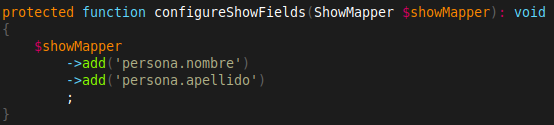
\includegraphics[width=1\linewidth]{image/show.png}
    \caption[Ejemplo de definición de campos a mostrar durante la creación/edición]{Ejemplo de definición de campos a mostrar durante la creación/edición.\newline \textbf{Fuente:} Elaboración propia.}
    \label{fig:image/show}
\end{figure}


\subsubsection{ABMs Compuestas}%
\label{ssub:admin_proyectadmin_proyecto}

En el sistema se separaron las ABM en dos tipos, en primer lugar se tienen aquellas que representan una relacion de 1-n con otros elementos del sistema,
es decir, actividades que pueden relizarse por muchas personas; en segundo lugar están las ABMs de actividades que son realizadas por sólo una persona.


En el primer caso, la implementación se hizo utilizando admins \textit{hijos}, una característica de \textbf{Sonata} que permite definir una jerarquía de clases admin que represente un
elemento \textit{padre} compuesto por uno o muchos elementos \textit{hijos}.

Cuando se asigna un admin como \textit{hijo} se obtienen rutas anidadas, de forma que se puede acceder a acciones del \textit{hijo} desde la vista del padre.
Ej: Una ruta
para acceder a un miembro en particular sería de la forma:\newline \textbf{/miembroproyecto/{id}/(show | edit)}\@.\newline\newline Cuando se accede a los
miembros de cada proyecto se obtienen rutas de la forma:\newline \textbf{/proyecto/{id}/miembroproyecto/{id}/(show | edit)},
\newline \textbf{/proyecto/{id}/miembroproyecto/list}\newline

A continuación se listan las ABM implementadas de esta forma:

\begin{itemize}
        \item Proyecto de Investigación
\item Proyecto de Extensión
\item Rol de Proyectos
\item Comisión de Consejo Superior
\item Práctica Profesional Supervisada
\item Actividad de Divulgación
\item Proyecto de Extensión
\item Curso de Extensión
\item Voluntariado
\item Programa

\end{itemize}

\myparagraph{Implementación de una ABM Compuesta: Proyecto}


En el admin de Proyecto se agregaron los siguientes campos en cada acción:

\begin{itemize}
    \item Lista: nombre del proyecto.
    \item Ver: nombre del proyecto
    \item Inserción: nombre y roles de proyecto.
\end{itemize}

Para asignar un admin como \textit{hijo} se debe configurar el servicio padre a través de un método denominado \textbf{addChild}. Como parámetros requiere el servicio
del admin a actuar de \textit{hijo} y el campo mediante el cual está relacionado al \textit{padre}.


Al agregar un admin como \textit{hijo} se generan las rutas anidadas (sección:~\ref{ssub:admin_proyectadmin_proyecto}), pero no se tiene una forma de acceder a
ellas desde la aplicación web\@. Una buena forma de solucionar este problema es, según la documentación de \textbf{Sonata}, agregar un menú en la barra superior
de la página que contenga botones mediante los cuales acceder a estas rutas.\parencite{sonata-childAdmin}


Para crear un proyecto se deben proporcionar los datos de nombre y roles. Los roles de proyecto están representados en la entidad en forma de Colección,
por lo tanto, se utilizó un tipo de formulario que permite la elección de opciones múltiples y, además, permite agregar nuevas instancias de
rol (figura~\ref{fig:image/proyecto-editar}).

\begin{figure}[H]
    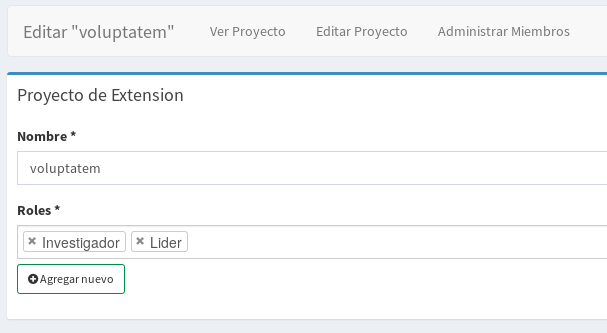
\includegraphics[width=1\linewidth]{image/edit-proyecto.png}
    \caption[Admin: Acción de  editar Proyectos]{Admin: Acción de  editar Proyectos.\newline \textbf{Fuente:} Elaboración propia, captura de pantalla de la aplicación web.}
    \label{fig:image/proyecto-editar}
\end{figure}
\newpage
\myparagraph{Miembro de Proyecto}%

Para la definición del admin de miembros de proyecto se lo estableció como un \textit{hijo} del admin Proyecto, esto es debido a que tiene sentido desde el punto
de vista de la relación que forman. Un proyecto estará integrado por muchos miembros, por lo tanto, al asignar a miembros de proyecto como admin \textit{hijo}
de Proyecto permite administrar los miembros desde la interfaz de proyectos. Al fin y al cabo, la clase admin de miembros no tiene sentido por sí sola.



\begin{figure}[H]
    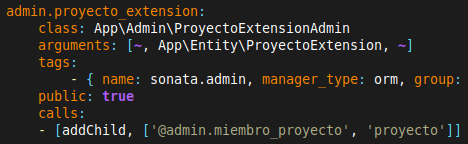
\includegraphics[width=1\linewidth]{image/addChild.png}
    \caption[Servicio admin de Proyecto de Extensión]{Servicio admin de Proyecto de Extensión.\newline \textbf{Fuente:} Elaboración propia, captura de pantalla de código fuente.}
    \label{fig:image/addChild}
\end{figure}

\myparagraph{Rol de proyecto}%

El admin de roles es muy básico pues solo contiene el campo de nombre. Por lo tanto, en cada una de sus acciones se agregó este único campo.


De igual manera que con \textbf{Proyecto}, se agregó al admin de miembros como \textit{hijo}. De esta forma se puede listar los miembros que cumplen cada rol en
particular.
Esto se logra mediante el método \textbf{addChild} (figura~\ref{fig:image/addChild}) y creando un menú del mismo tipo que el definido en el admin de proyectos.

\subsubsection{ABMs Simples y admins \textit{hijos}}%
\label{ssub:ambs_simples}

En el caso que una actividad solo fuera completada por una persona, o se tratase de un admin \textit{hijo}, la definición del admin solo contendría los
datos de la persona y la actividad\@. Las ABMs implementadas de esta manera se listan a continuación:

\begin{itemize}
        \item Asambleista
\item Consejero Superior
\item Director de Instituto
\item Coordinador de Materia
\item Director de Carrera
\item Miembro de Proyecto
\item Miembro de Comisión de Consejo Superior
\item Miembro de Práctica Profesional Supervisada
\item Rector
\item Miembro de Curso de Extension
\item Miembro de Actividad de Divulgación
\item Miembro de Pasantia
\item Miembro de Voluntariado
\item Responsable de Area
\item Miembro de Programa
\item Vinculador
\item Vice Rector
\item Secretario
\item Beca Befat
\item Movilidad Conurbano Sur
\item Publicacion
\item Movilidad RTF
\item Sub-Secretario

\end{itemize}

\myparagraph{Implementación ABM Simple: Publicación}

Se implementó la entidad extendiendo de la clase \textbf{Actividad} y se definió el admin de manera que:

\begin{itemize}
    \item La acción de crear una publicación requiere especificar la persona, la fecha de inicio y la fecha de fin de la actividad.
    \item Las acciones de listar y visualizar el elemento muestran los datos de la persona y la actividad.
\end{itemize}

Mediante la función \textit{configureFormFields} se establecieron los campos a llenar durante la creación de una Publicación.

\begin{lstlisting}[caption={Definición de campos durante la creación de Publicaciones.\\Fuente: Elaboración propia}]
public function configureFormFields(
    FormMapper $formMapper
): void {
    $formMapper
        ->add('persona', ModelListType::class)
        ->add('inicio', DatePickerType::class)
        ->add('fin', DatePickerType::class)
        ;
}
\end{lstlisting}

Se utilizó un tipo de formulario de \textbf{Sonata} llamado \textbf{ModelListType}, que permite seleccionar las personas a través de una lista y se agregó
un elemento \textbf{Datepicker} para especificar
las fechas\@. Además, se separó la funcionalidad común en un Trait de PHP de manera que si se necesita algo en específico, se puede sobrescribir los métodos
en la clase admin base.




\subsection{Librerías}%
\label{sub:librerias}

Si bien en muchos de los casos las librerías utilizadas en el desarrollo fueron configuradas por el componente~\textbf{Flex}  de \textbf{Symfony}, algunos paquetes
requirieron de una configuración más compleja y son los aquí listados.

\subsubsection{Instalación y Configuración de Sonata-User}%
\label{ssub:instalacion_y_configuración_de_sonata-user}

Esta librería integra el componente \textbf{FOSUser} de \textbf{Symfony} con \textbf{Sonata Admin} y agrega algunas características adicionales.




Para su instalación es necesario tener FOSUser instalado y configurado además de SonataAdmin y SonataEasyExtends\@.
Para este proceso se siguieron los pasos establecidos en la documentación de \textbf{Sonata-User}~\parencite{sonata-user}

\begin{figure}[H]
    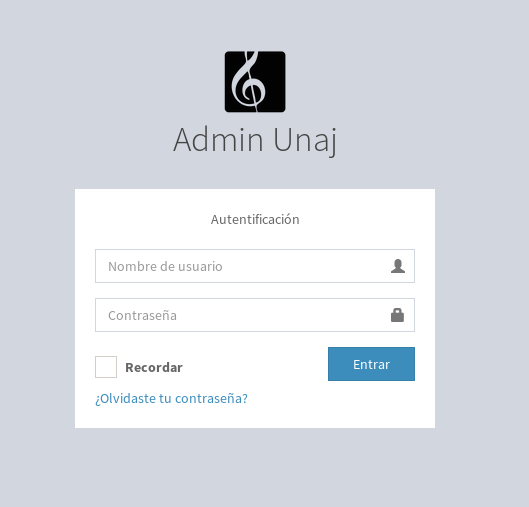
\includegraphics[width=1\linewidth]{image/adminLogin.png}
    \caption{Pantalla de login de Sonata-User\newline \textbf{Fuente:} Elaboración propia, captura de pantalla de la aplicación web}
    \label{fig:image/adminLogin}
\end{figure}

Configuración básica: Sonata User involucra varias librerías y elementos del sistema que deben ser configurados adecuadamente, estos son:

\begin{itemize}
    \item \textbf{Doctrine:} se debe definir el mapeo de entidades necesarias para el funcionamiento de la librería.
    \item \textbf{FOSUser:} se requiere especificar entidades y servicios para la administración de usuarios y grupos.
    \item \textbf{Security:} es necesario configurar la autenticación de usuarios y el control de acceso.
    \item \textbf{Routing:} se debe agregar información necesaria para la generación de rutas.
    \item \textbf{Sonata-User:} configuración que define el tipo de datos y las clases que definen la estructura de los datos de usuarios y grupos.
\end{itemize}



Como primer paso para la instalación y configuración de Sonata-User, se agregó la librería FOSUser y Sonata-User a través del gestor de paquetes Composer,
luego se comenzó con la configuración:

\paragraph{Sonata-User}~\newline

Se especificó a Sonata-User que los datos son administrados por un ORM.

\begin{lstlisting}[caption={archivo de configuración de sonata-user\\Fuente: \sonatainstallation.}]
#src/config/packages/sonata_user.yaml

sonata_user:
    manager_type: orm

\end{lstlisting}

\paragraph{FOSUser}~\newline

En cuanto a FOSUser se definió el driver de base de datos como ORM y el sistema de autenticación que utilizará\@. También se especificaron clases base
proporcionadas por Sonata-User, que serán utilizadas para la generación de las entidades finales de usuario y grupo\@. Por último, se definen los servicios
que administran estas entidades e información sobre el servicio de correo.

\begin{lstlisting}[caption={archivo de configuración de FOSUser\\ Fuente: \sonatainstallation.}]
#src/config/packages/fos_user.yaml

fos_user:
    db_driver: orm
    firewall_name: main
    user_class: Sonata\UserBundle\Entity\BaseUser
    group:
      group_class: Sonata\UserBundle\Entity\BaseGroup

      group_manager: sonata.user.orm.group_manager
    service:
      user_manager: sonata.user.orm.user_manager

    from_email:
        address: "test@domain.com"
        sender_name: "test@domain.com"

\end{lstlisting}

\myparagraph{Doctrine}


La única configuración necesaria para el ORM es la definición explícita de cada una de las entidades mapeadas.
Doctrine cuenta con una característica llamada auto mapping, que permite cargar la configuración de entidades almacenadas bajo el directorio Entity/
de cada uno de los bundles.
Para la configuración de doctrine, cada entidad utilizada por Sonata-User y FOSUser debe estar definida en su archivo de configuración; pero dado que se
tiene habilitado la función de auto mapping y cada entidad está bajo un directorio de nombre “Entity” no es necesario agregar nada a la configuración existente.

\myparagraph{Routing}


Se agregaron las configuraciones de las rutas necesarias para ambas librerías.



\begin{lstlisting}[caption={archivo de configuración de rutas de FOSUser\\Fuente: \sonatainstallation.}]
#src/config/routes/fos_user.yaml

fos_user:
    resource: "@FOSUserBundle/Resources/config/routing/all.xml"
\end{lstlisting}

\begin{lstlisting}[caption={archivo de configuración de rutas de sonata-user\\Fuente: \sonatainstallation.}]
#src/config/routes/sonata_user.yaml

sonata_user_admin_security:
    resource: '@SonataUserBundle/Resources/config/routing/admin_security.xml'
    prefix: /admin

sonata_user_admin_resetting:
    resource: '@SonataUserBundle/Resources/config/routing/admin_resetting.xml'
    prefix: /admin/resetting

\end{lstlisting}

\myparagraph{Security}

En cuanto a la configuración de seguridad, se definieron dos sistemas de autenticación (denominados firewall)\@. Uno se encargará de administrar la seguridad en
los usuarios admin y el otro en usuarios básicos.

\begin{lstlisting}[caption={Firewall para el área admin del sistema.\\Fuente: \sonatainstallation.}]
#src/config/packages/security.yaml

# -> custom firewall for the admin area of the URL
        admin:
            pattern:            /admin(.*)
            context:            user
            form_login:
                provider:       fos_userbundle
                login_path:     /admin/login
                use_forward:    false
                check_path:     /admin/login_check
                failure_path:   null
                default_target_path: /admin/dashboard
            logout:
                path:           /admin/logout
                target:         /admin/login
            anonymous:          true
\end{lstlisting}

\newpage
\begin{lstlisting}[caption={Firewall para el área de registro y login de usuarios básicos.\\Fuente: \sonatainstallation.}]
#src/config/packages/security.yaml
        main:
            pattern:             .*
            context:             user
            form_login:
                provider:       fos_userbundle
                login_path:     /login
                use_forward:    false
                check_path:     /login_check
                failure_path:   null
            logout:             true
            anonymous:          true
\end{lstlisting}

\noindent
Además se especificó la jerarquía de roles y proveedor de usuarios:

\begin{lstlisting}[caption={Jerarquía de roles, tipo de encriptación y proveedor de usuarios\\Fuente: \sonatainstallation}]
    role_hierarchy:
        ROLE_ADMIN:       [ROLE_USER, ROLE_SONATA_ADMIN]
        ROLE_SUPER_ADMIN: [ROLE_ADMIN, ROLE_ALLOWED_TO_SWITCH]
        SONATA:
            - ROLE_SONATA_PAGE_ADMIN_PAGE_EDIT

    providers:
        fos_userbundle:
            id: fos_user.user_provider.username

    encoders:
        FOS\UserBundle\Model\UserInterface: bcrypt
\end{lstlisting}

\newpage
Por último, se define el control de acceso de manera que se pueda ingresar anónimamente a cada página de registro, inicio de sesión, reinicio de contraseña,
etc.
También se especifica qué roles tienen permitido ingresar a la parte de administración del sistema.

\begin{figure}[h]
    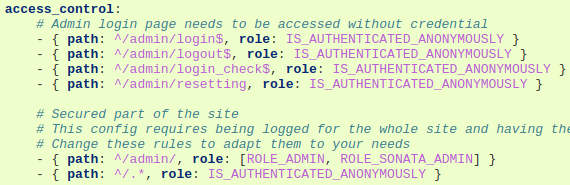
\includegraphics[width=1\linewidth]{image/acl.png}
    \caption{Control de acceso\newline \textbf{Fuente:} Recuperado de https://sonata-project.org/bundles/user/master/doc/reference/installation.html}
    \label{fig:image/acl}
\end{figure}

\myparagraph{Generación de entidades finales}

A partir de esta configuración se generaron las entidades de usuario y grupo mediante el comando:

\begin{lstlisting}
bin/console sonata:easy-extends:generate SonataUserBundle --dest=src --namespace_prefix=App
\end{lstlisting}


Esto da como resultado un directorio en \textbf{Application\textbackslash Sonata\textbackslash UserBundle} el cual contiene las entidades a utilizar por las librerías.
Por último, se configuró Sonata-User y FOSUser para que utilicen las nuevas entidades:

\begin{lstlisting}[caption={Archivo de configuración de Sonata-User.\\Fuente: \sonatainstallation}]
#src/config/packages/sonata_user.yaml

sonata_user:
  manager_type: orm
  class:
        user: App\Application\Sonata\UserBundle\Entity\User
        group: App\Application\Sonata\UserBundle\Entity\Group

\end{lstlisting}

\newpage
\begin{lstlisting}[caption=Archivo de configuración de FOSUser.\\Fuente: \sonatainstallation]
#src/config/packages/fos_user.yaml

fos_user:
    db_driver: orm # other valid values are 'mongodb' and 'couchdb'
    firewall_name: main
    user_class: App\Application\Sonata\UserBundle\Entity\User
    group:
      group_class:   App\Application\Sonata\UserBundle\Entity\Group
      group_manager: sonata.user.orm.group_manager
    service:
      user_manager: sonata.user.orm.user_manager

    from_email:
        address: "test@domain.com"
        sender_name: "test@domain.com"

\end{lstlisting}

\subsubsection{API-Platform}%
\label{ssub:api_platform}

Para la instalación de esta librería sólo es necesario agregarla a través de \textbf{Composer} y Flex se hace cargo de la configuración\@. Luego de realizado
esto, se configuró las entidades a exponer, que en este caso serían todas las entidades que representan datos en el sistema.


API-Platform permite definir las entidades a utilizar durante el proceso de serialización mediante anotaciones o archivos de configuración. Por defecto,
este componente serializa todos los campos y todas aquellas funciones que retornen algún valor\@. Probablemente se tengan entidades con funciones o datos
que no se quieran exponer a los usuarios. Además, se pueden encontrar referencias circulares entre algunas entidades, que fue lo que sucedió entre miembros
y roles de proyecto (un miembro tiene un rol, y un rol tiene muchos miembros)\@.  Por este motivo, se decidió configurar la información que es expuesta a
través de estas entidades.

\myparagraph{El proceso de serialización}


La serialización es el proceso de convertir estructuras de datos u objetos en un formato que puede ser almacenado (por ejemplo, en un archivo o búfer de memoria)
o transmitido (por ejemplo, a través una conexión de red) y reconstruido luego (posiblemente en un entorno diferente).~\parencite{serialization}

\begin{figure}[H]
    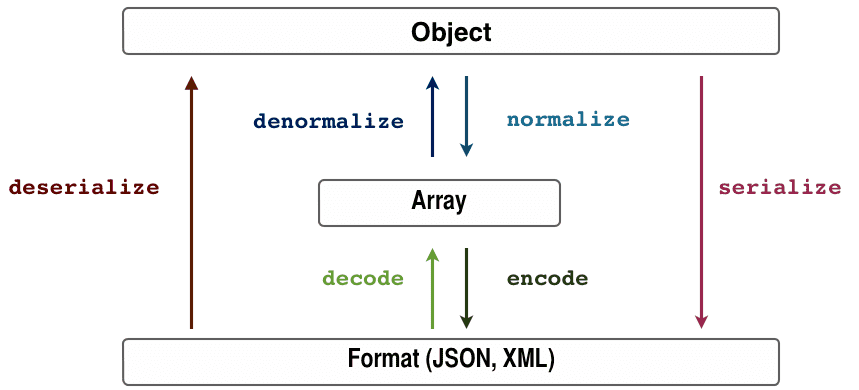
\includegraphics[width=1\linewidth]{image/serializationWorkflow.png}
    \caption{El proceso de serialización\newline \textbf{Fuente:} Recuperado de~\url{https://api-platform.com/docs/core/serialization/}}
    \label{fig:image/serializationWorkflow}
\end{figure}

En \textbf{Symfony} esto es logrado a través del componente \textbf{Serializer}. El proceso en sí, sigue el esquema presentado en la figura
\ref{fig:image/serializationWorkflow}\@.
Para la conversión primero se convierte el objeto en un \textit{array} (proceso denominado
normalización) y luego se convierte al formato específico que se necesite (a este proceso se lo llama codificación).

API-Platform permite modificar la información que se expone a los usuarios mediante grupos de \textit{serialización} y \textit{deserialización}\@. A través del uso de anotaciones
en cada propiedad de la entidad se puede definir si agregar la propiedad al proceso de normalización o no dependiendo de la acción que se esté realizando.
Si se desean funciones más complejas, es posible definir \textit{normalizadores} y \textit{codificadores} personalizados o decorar \textit{normalizadores} existentes.
~\parencite{api-platform-serialization}

\myparagraph{Modificación del proceso de serialización}

Mediante anotaciones se agregó cada propiedad relevante a cada acción en particular y se omitieron aquellas propiedades o funciones que no necesitan estar
presentes o que no se desean exponer a los usuarios.

Al definir un grupo de serialización se logra que, al agregar una propiedad al contexto de normalización, sólo se serialice las propiedades pertenecientes
al grupo en cuestión. Esto significa, que si se agrega una relación al contexto de normalización, se serializarán los campos de la entidad relacionada
que pertenezcan a dicho grupo.


\subsubsection{Guzzle y EightPointsGuzzle}%
\label{ssub:guzzle}

Guzzle es una librería que facilita la interacción con servicios web, al proveer métodos simples para realizar solicitudes \textbf{HTTP}\@. Su funcionamiento consiste en la creación
de un objeto llamado \textbf{cliente}, el cual provee acceso al servicio web a utilizar.


Eightpoints integra Guzzle con Symfony y permite definir un cliente como servicio de manera que sea posible utilizarlo en cualquier parte de la aplicación.


Se utilizaron estas dos librarías para configurar los servicios web a integrar con RUDA. Su configuración requiere de la ruta base de la API para funcionar y es posible definir
diversas opciones como headers y autenticación.


Se definió un cliente Guzzle para el servicio web de mapuche definiendo su ruta base, método de autenticación y headers. Como autenticación se utilizó HTTP digest y se definieron
 headers que definen el formato a utilizar como \textbf{json}.


\subsection{Vista de Persona}
\label{sub:vista_persona}
Se creó una vista mediante la cual se pueda acceder a la información de cada persona y a la lista de actividades en las que se encuentra involucrada. Su
implementación se basó en la iteración de la colección de actividades  de la persona y la generación de html mediante \textbf{Twig}\@.
Como último paso se agregó algo de estilo mediante \textbf{CSS} y una simple animación en \textbf{Javascript}.


% TODO   franco continuar vie 01 nov 2019 20:37:16 -03

\begin{figure}[h]
    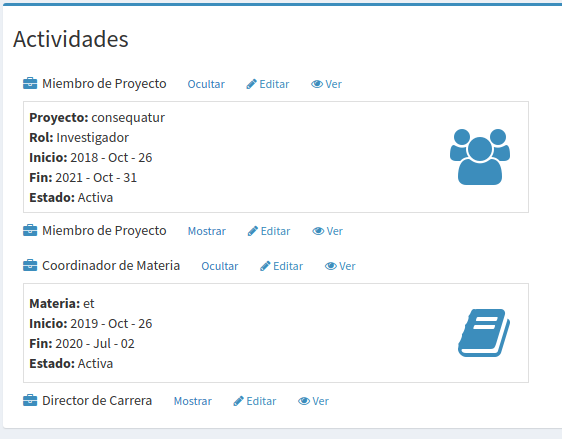
\includegraphics[width=1\linewidth]{image/vista_persona.png}
    \caption{Listado de actividades.\newline \textbf{Fuente:} Elaboración propia, captura de pantalla de aplicación web.}
    \label{fig:image/vista_persona}
\end{figure}


\begin{figure}[h]
    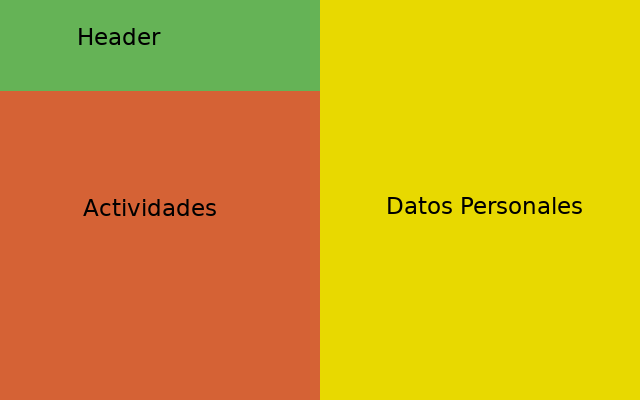
\includegraphics[width=1\linewidth]{image/grid.png}
    \caption{Distribución de columnas y filas.\newline \textbf{Fuente:} Elaboración propia.}
    \label{fig:image/grid}
\end{figure}




\section{Conclusión}
\label{sec:conclusion}
El hecho de no contar con un sistema que almacene la información de cada
actividad extracurricular realizada por las personas de la UNAJ presenta
un problema para la institución y sus integrantes\@. Estos datos
no solo son valiosos debido a propósitos administrativos, sino que cada una de
estas actividades le otorga un valor agregado a la historia académica del
estudiante y deberían ser registradas al igual que sus
materias y calificaciones.


En cuanto al desarrollo, se consiguió implementar una interfaz web que ayudará
a la administración de estos datos. Será posible solicitar la información de
una determinada persona y obtener una lista sus actividades extracurriculares y cargos\@.
Cada actividad contará con una interfaz administrativa, lo que
permitirá agregar personas al sistema y asignarle las actividades o cargos
que se requieran\@. Además, se terminó por definir un servicio REST que
obtiene parte de su información del sistema \textbf{Mapuche} e integra
los datos de ambos sistemas\@.


Con respecto al sistema \textbf{Guaraní}, no se alcanzó a implementar la
integración por razones de tiempo, ya que se debe ajustar el sistema RUDA para
que los dos tipos de datos de personas coexistan entre sí: una persona puede
estar trabajando en la universidad, es decir, registrada en el sistema
\textbf{Mapuche} y al mismo tiempo estudiando. Estos dos datos deben
vincularse para representar una sola persona y además, indicar estos tipos
de situaciones.

Contar con esta información puede dar lugar a análisis de datos,
estadística e incluso el desarrollo de otros proyectos. Será posible,
por ejemplo, identificar alumnos que sean muy activos en áreas de
investigación, lo que podría dar lugar a un diferente tipo de orientación
o tutoría para un mejor aprovechamiento de sus habilidades\@. Además de lo mencionado, quizás
en un futuro se pueda listar esta información en un comprobante o anexo al título universitario
de manera de resaltar los méritos de la persona.

Mejorar los procesos de administración de la información de la Universidad es muy necesario
y útil a futuro, ya que beneficia a todos los que la integran.

\section{Reflexión}%
\label{sec:reflexión}

Aprender un \textit{framework} no resulta ser un proceso trivial, requiere de aprender los
distintos componentes que lo conforman y en parte, su funcionamiento interno\@. Es necesario
utilizar y leer código con el que no se está familiarizado y que pasó por muchas revisiones
hasta llegar al público.

Trabajar con código de terceros es una buena manera de ejercitar la habilidad de \textit{leer}
código\@. Esta habilidad puede abrir la puerta a contribuciones a proyectos open source o
personales.

Durante el transcurso de esta PPS, no sólo aprendí a trabajar con un nuevo \textit{framework},
también me familiaricé con diferentes flujos de trabajo y herramientas\@. Definitivamente es
el proyecto más grande del que formé parte y, por consiguiente, el que más aprendizaje me otorgó.

El proyecto en sí me presentó un desafío por el hecho de tener que sobrellevar el desarrollo
del sistema con la escritura y organización del documento\@. Escribir un documento académico
puede volverse una tarea bastante desorganizada (al menos en mi caso) utilizando procesadores
de texto comunes, esto es por que ni bien crece el documento, crece la cantidad de secciones
que se deben modificar y mantener\@. Esto es lo que me llevó a aprender el sistema {\LaTeX}\@.
El mismo solucionó gran parte de mis problemas de organización, al poder
separar el documento en archivos individuales para cada sección\@. Además, la inserción de
gráficos o secciones de código están manejadas internamente y no hay necesidad de
preocuparse por los
epígrafes, ya que son enumerados automáticamente\@. Como si esto fuera poco {\LaTeX} permite
definir funciones: esto hace posible programar diferentes tipos de contenido reutilizable en todo el
documento.


Por otro lado, este proyecto me llevó a descubrir el área en la cual quiero desenvolverme como
futuro Ingeniero, me interesa bastante la optimización y/o automatización de procesos de todo
tipo. Quizás también relacionado con la programación o administración de sistemas\@. Previo a
este proyecto no tenía una idea bastante formada respecto a este tema, así que me fue de gran
ayuda.\newline


\noindent\fbox{
    \parbox[t][]{\textwidth}{
        \textbf{REFLEXIÓN SOBRE LA PRÁCTICA PROFESIONAL SUPERVISADA COMO ESPACIO DE FORMACIÓN:}\\~\\



        Aprender un \textit{framework} no resulta ser un proceso trivial, requiere de aprender los
        distintos componentes que lo conforman y en parte, su funcionamiento interno\@. Es necesario
        utilizar y leer código con el que no se está familiarizado y que pasó por muchas revisiones
        hasta llegar al público.

        Trabajar con código de terceros es una buena manera de ejercitar la habilidad de \textit{leer}
        código\@. Esta habilidad puede abrir la puerta a contribuciones a proyectos open source o
        personales.

        Durante el transcurso de esta PPS, no sólo aprendí a trabajar con un nuevo \textit{framework},
        también me familiaricé con diferentes flujos de trabajo y herramientas\@. Definitivamente es
        el proyecto más grande del que formé parte y, por consiguiente, el que más aprendizaje me otorgó.

        El proyecto en sí me presentó un desafío por el hecho de tener que sobrellevar el desarrollo
        del sistema con la escritura y organización del documento\@. Escribir un documento académico
        puede volverse una tarea bastante desorganizada (al menos en mi caso) utilizando procesadores
        de texto comunes, esto es por que ni bien crece el documento, crece la cantidad de secciones
        que se deben modificar y mantener\@. Esto es lo que me llevó a aprender el sistema {\LaTeX}\@.
        El mismo solucionó gran parte de mis problemas de organización, al poder
        separar el documento en archivos individuales para cada sección\@. Además, la inserción de
        gráficos o secciones de código están manejadas internamente y no hay necesidad de
        preocuparse por los
        epígrafes, ya que son enumerados automáticamente\@. Como si esto fuera poco {\LaTeX} permite
        definir funciones: esto hace posible programar diferentes tipos de contenido reutilizable en todo el
        documento.


        Por otro lado, este proyecto me llevó a descubrir el área en la cual quiero desenvolverme como
        futuro Ingeniero, me interesa bastante la optimización y/o automatización de procesos de todo
        tipo. Quizás también relacionado con la programación o administración de sistemas\@. Previo a
        este proyecto no tenía una idea bastante formada respecto a este tema, así que me fue de gran
        ayuda.
    }
}



\begin{framed}

        \noindent\textbf{REFLEXIÓN SOBRE LA PRÁCTICA PROFESIONAL SUPERVISADA COMO ESPACIO DE FORMACIÓN:}\\~\\


        Aprender un \textit{framework} no resulta ser un proceso trivial, requiere de aprender los
        distintos componentes que lo conforman y en parte, su funcionamiento interno\@. Es necesario
        utilizar y leer código con el que no se está familiarizado y que pasó por muchas revisiones
        hasta llegar al público.

        Trabajar con código de terceros es una buena manera de ejercitar la habilidad de \textit{leer}
        código\@. Esta habilidad puede abrir la puerta a contribuciones a proyectos open source o
        personales.

        Durante el transcurso de esta PPS, no sólo aprendí a trabajar con un nuevo \textit{framework},
        también me familiaricé con diferentes flujos de trabajo y herramientas\@. Definitivamente es
        el proyecto más grande del que formé parte y, por consiguiente, el que más aprendizaje me otorgó.

        El proyecto en sí me presentó un desafío por el hecho de tener que sobrellevar el desarrollo
        del sistema con la escritura y organización del documento\@. Escribir un documento académico
        puede volverse una tarea bastante desorganizada (al menos en mi caso) utilizando procesadores
        de texto comunes, esto es por que ni bien crece el documento, crece la cantidad de secciones
        que se deben modificar y mantener\@. Esto es lo que me llevó a aprender el sistema {\LaTeX}\@.
        El mismo solucionó gran parte de mis problemas de organización, al poder
        separar el documento en archivos individuales para cada sección\@. Además, la inserción de
        gráficos o secciones de código están manejadas internamente y no hay necesidad de
        preocuparse por los
        epígrafes, ya que son enumerados automáticamente\@. Como si esto fuera poco {\LaTeX} permite
        definir funciones: esto hace posible programar diferentes tipos de contenido reutilizable en todo el
        documento.


        Por otro lado, este proyecto me llevó a descubrir el área en la cual quiero desenvolverme como
        futuro Ingeniero, me interesa bastante la optimización y/o automatización de procesos de todo
        tipo. Quizás también relacionado con la programación o administración de sistemas\@. Previo a
        este proyecto no tenía una idea bastante formada respecto a este tema, así que me fue de gran
        ayuda.

\end{framed}

\vfill
\noindent\begin{tabular}{|P{3.3cm}|P{3.3cm}|P{3.3cm}|P{3.3cm}|}
\hline
Firma Estudiante: & Firma Docente Supervisor: & Firma docente tutor TAPTA: & Firma tutor Organizacional: \\
~ & ~ & ~ & ~ \\
\hline
\end{tabular}


\newpage
\nocite{*}
\printbibliography

\newpage

\listoffigures




\end{document}
